\newpage
\section{TypeSafe Enum Pattern}

The enums are type-safe means that an enum has its own namespace, we can’t assign any other value other than specified in enum constants. Additionally, an enum is a reference type, which means that it behaves more like a class or an interface. As a programmer, we can create methods and variables inside the enum declaration.
\subsection{Class Diagram}

\begin{figure}[h]
\centering
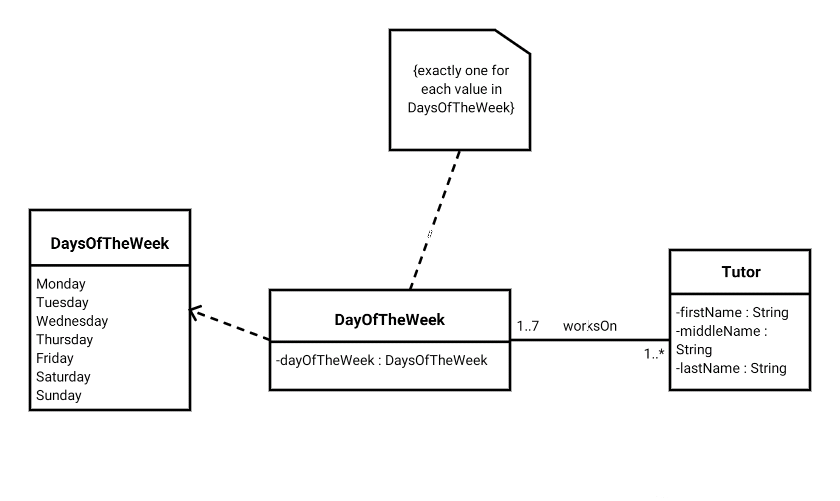
\includegraphics[scale=0.5]{enum}
\caption{Class Diagram of TypeSafeEnum Pattern}
\end{figure}

\newpage
\subsection{Source Code (Java)}

\subsubsection{Suit Class}

\begin{minted}{java}
public class Suit {
    private final String name;
    public static final Suit CLUBS = new Suit("clubs");
    public static final Suit DIAMONDS = new Suit("diamonds");
    public static final Suit HEARTS = new Suit("hearts");
    public static final Suit SPADES = new Suit("spades");
    private Suit(String name) {
        this.name = name;
    }
    public String toString() {
        return name;
    }
}
\end{minted}

\subsubsection{Suit Enum}

\begin{minted}{java}
public enum Suit {
    CLUBS("clubs"), DIAMONDS("diamonds"), HEARTS("hearts"), SPADES("spades");
    private final String name;
    private Suit(String name) {
        this.name = name;
    }
}
\end{minted}